\documentclass{article}

\usepackage{graphicx}
\usepackage{tikz}
\usepackage{tikzsymbols}
\usetikzlibrary{calc,patterns,shapes.geometric}
\pagestyle{empty}
\usepackage[margin=0pt]{geometry}
\geometry{papersize={14in,12in}}

\def\centerarc[#1](#2)(#3:#4:#5){\draw[#1] ($(#2)+({#5*cos(#3)},{#5*sin(#3)})$) arc (#3:#4:#5);}

\begin{document}
	\begin{figure}
		\centering
		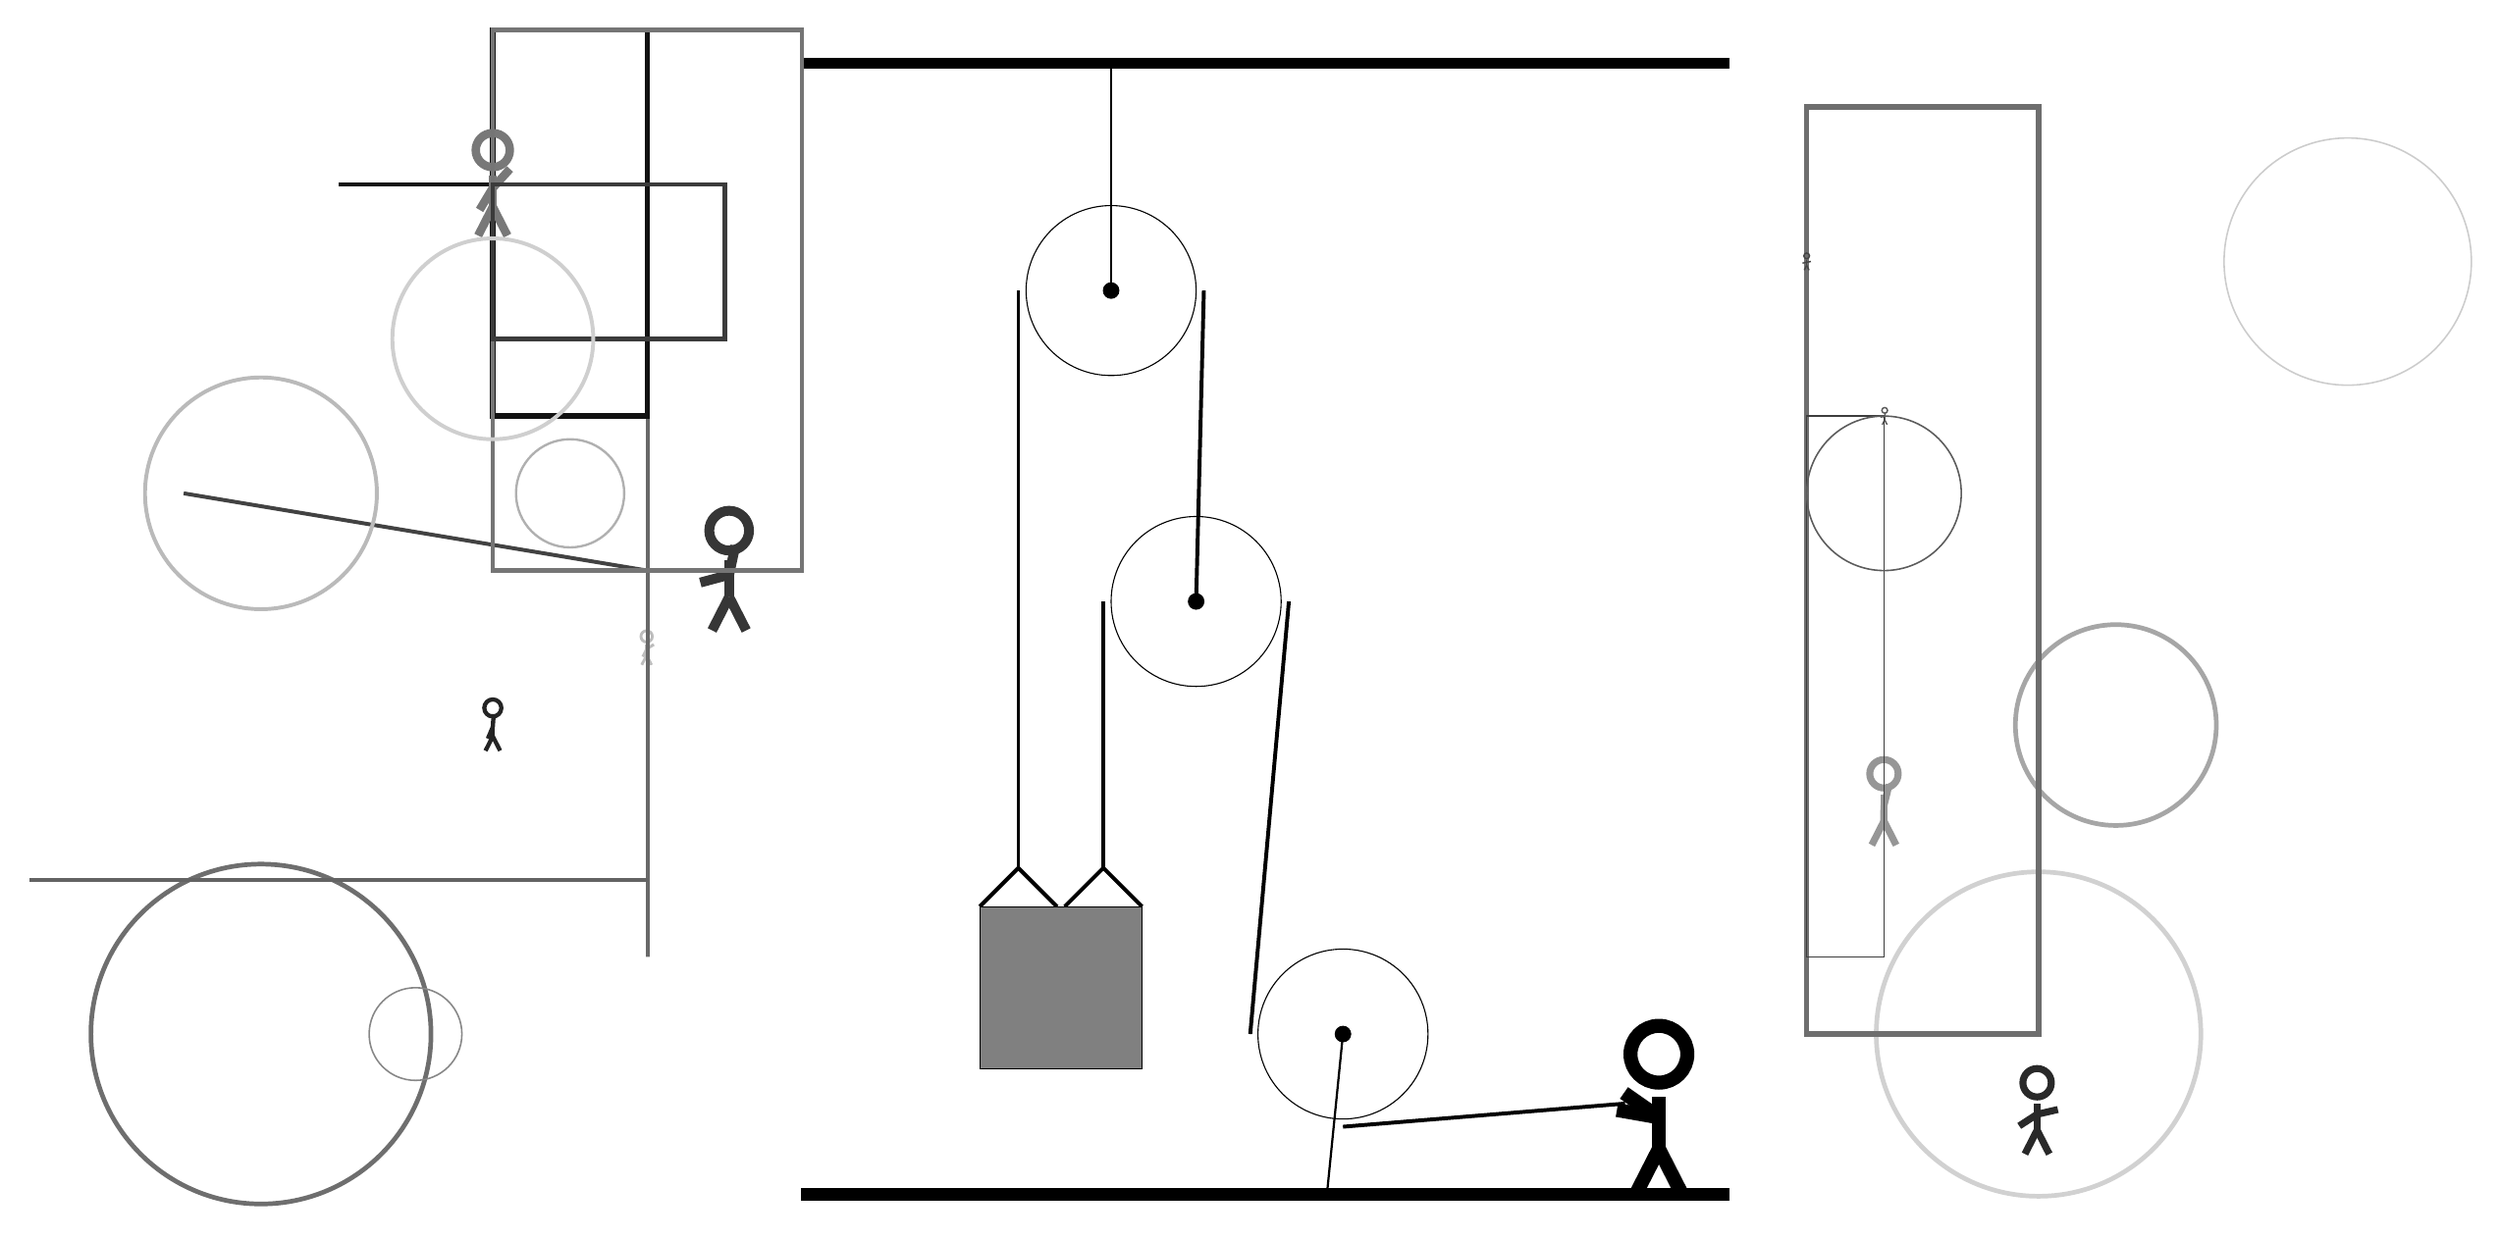
\begin{tikzpicture}
			%%%%% START %%%%%
			
			\draw[fill=black] (-2, 11.5) rectangle (10, 11.625);
			
			\draw [line width=0.6mm, color=black!35](15, 3) circle (1.3);
			
			\node[line width=0.3mm, color=black!41] at (12, 2) {\Strichmaxerl[5][89][76]};
			\draw [line width=0.3mm, color=black!31](-5, 6) circle (0.7);
			\node[line width=0.6mm, color=black!26] at (-4, 4) {\Strichmaxerl[2][64][32]};
			
			\draw [line width=0.6mm, color=black!18](14, -1) circle (2.1);
			\draw [line width=0.6mm, color=black!57](-9, -1) circle (2.2);
			\draw[line width=0.2mm, color=black!73] (11, 0) rectangle (11, -1);
			\draw[line width=0.5mm, color=black!59] (-4, 9) rectangle (-4, 0);
			\draw[line width=0.7mm, color=black!57] (11, 11) rectangle (14, -1);
			\draw[line width=0.5mm, color=black!74](-4, 5) -- (-10, 6);
			\draw[line width=0.5mm, color=black!92](-4, 10) -- (-8, 10);
			\node[line width=0.2mm, color=black!65] at (12, 7) {\Strichmaxerl[1][5][82]};
			\node[line width=0.7mm, color=black!86] at (-6, 3) {\Strichmaxerl[3][67][86]};
			
			\draw[line width=0.2mm, color=black!76] (11, 0) rectangle (12, 7);
			\node[line width=0.4mm, color=black!79] at (-3, 5) {\Strichmaxerl[7][15][78]};
			\node[line width=0.3mm, color=black!73] at (11, 9) {\Strichmaxerl[1][13][9]};
			
			\draw[line width=0.7mm, color=black!93] (-4, 7) rectangle (-6, 12);
			\draw [line width=0.5mm, color=black!27](-9, 6) circle (1.5);
			\node[line width=0.6mm, color=black!84] at (14, -2) {\Strichmaxerl[5][33][13]};
			\node[line width=0.4mm, color=black!53] at (-6, 10) {\Strichmaxerl[6][59][48]};
			\draw[line width=0.6mm, color=black!54] (-2, 12) rectangle (-6, 5);
			
			\draw [line width=0.2mm, color=black!20](18, 9) circle (1.6);
			\draw[line width=0.5mm, color=black!61](-4, 1) -- (-12, 1);
			\draw [line width=0.2mm, color=black!47](-7, -1) circle (0.6);
			\draw[line width=0.6mm, color=black!77] (-3, 8) rectangle (-6, 10);
			\draw [line width=0.5mm, color=black!19](-6, 8) circle (1.3);
			\draw [line width=0.2mm, color=black!64](12, 6) circle (1.0);
			
			\draw (2, 8.625) circle (1.1);
			\draw[fill=black] (2, 8.625) circle (0.1);
			\draw[thick] (2, 8.625) -- (2, 11.5);
			
			\draw (3.1, 4.6) circle (1.1);
			\draw[fill=black] (3.1, 4.6) circle (0.1);
			
			\draw (5, -1) circle (1.1);
			\draw[fill=black] (5, -1) circle (0.1);
			\draw[thick] (5, -1) -- (4.8, -3);
			
			\draw[line width = 0.5mm]  (0.3, 0.65) -- (0.8, 1.15) -- (1.3, 0.65);
			\draw[line width = 0.5mm]  (1.4, 0.65) -- (1.9, 1.15) -- (2.4, 0.65);
			\draw[fill=black!50] (0.3, 0.65) rectangle (2.4, -1.45);
			
			\draw[line width = 0.5mm] (0.8, 8.625) -- (0.8, 1.15);
			\centerarc[line width = 0.5mm](2, 8.625)(0:180:1.2000000000000002);
			\draw[line width = 0.5mm] (3.2, 8.625) -- (3.1, 4.6);
			\draw[line width = 0.5mm] (1.9, 4.6) -- (1.9, 1.15);
			\centerarc[line width = 0.5mm](3.1, 4.6)(0:180:1.2000000000000002);
			\draw[line width = 0.5mm] (4.3, 4.6) -- (3.8, -1);
			\centerarc[line width = 0.5mm](5, -1)(180:270:1.2000000000000002);
			\draw[line width = 0.5mm] (5, -2.2) -- (8.65, -1.9);
			
			\node at (9, -2) {\Strichmaxerl[10][-35][170]};
			
			\draw[fill=black] (-2, -3) rectangle (10, -3.15);
			
			%%%%% END %%%%%
		\end{tikzpicture}
	\end{figure}	
\end{document}